\documentclass[preprint,12pt,a4]{standalone}
\usepackage{geometry}   % my added package "geometry"
\geometry{letterpaper,tmargin=1in,bmargin=1in,lmargin=2.5cm,rmargin=2.5cm}
\usepackage{tikz}
\usetikzlibrary{calc,patterns,arrows.meta,shapes.arrows,intersections,positioning}
\usetikzlibrary{decorations.pathmorphing,backgrounds,fit,petri}
\usepackage{standalone}
%
\begin{document}
	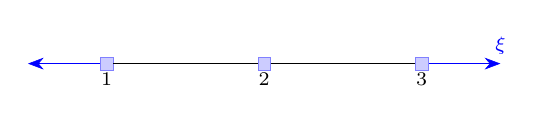
\begin{tikzpicture} [{place/.style={rectangle,draw=blue!50,fill=blue!20,ultra thin,inner sep=0.8mm}},{place2/.style={circle,draw=black!50,ultra thin,inner sep=0.8mm}},{linest/.style={color=gray,ultra thin}}]
		%axes
		\draw [{Stealth[length=2mm]}-{Stealth[length=2mm]}, help lines,blue] (5,0)node[above,font=\scriptsize]{$\xi$} -- (0,0)--(-1,0);
		%%element Nodes
		\node at (0.0,0.0) [place] (1) {};
		\node at (2.0,0.0) [place] (2) {};
		\node at (4.0,0.0) [place] (3) {};
		

		%%element border
		\draw [-] (1)node[below,font=\scriptsize]{$1$} --(2)node[below,font=\scriptsize]{$2$}--(3)node[below,font=\scriptsize]{$3$};
	\end{tikzpicture}
\end{document}